In addition to the purposes reviewed in \cref{sec:purposes}, most applications of modular deep learning revolve around transfer learning. In particular, the two main purposes are: \textbf{1}) \textit{parameter-efficient} fine-tuning (\S~\ref{ssec:eff_ft}), which achieves superior efficiency, prevents negative interference, and enables zero-shot transfer; and \textbf{2}) zero/few-shot generalisation to new tasks (\S~\ref{ssec:task_gen}).

%The main purpose of this section is to demonstrate how the main concepts surveyed in this work are leveraged to boost applications across several application areas, what content can be stored in the modules, as well as to make connections between theory and practice of modular deep learning. The goal is not to exhaustively list all the deep learning papers that relied on modular design but rather emphasise salient patterns and (dis)similarities in the literature.

\subsection{Parameter-Efficient Fine-tuning} 
\label{ssec:eff_ft}
Regardless of the application area, one of the principal uses of modules has been to boost parameter efficiency and decrease model storage requirements of fine-tuning, eschewing so-called \textit{full model fine-tuning} which requires storing a separate copy of the full model per task \citep{Howard2018ulmfit,Devlin:2019bert}, see \S\ref{sec:training:posthoc}. In the simplest formulation, all task-specific updates are pushed to the parameters of the lightweight modules, while the parameters of the large base model are kept \textit{frozen} throughout task fine-tuning. The modules then store \textit{task-specific knowledge} that can be composed with the `general-purpose' knowledge of the base model to adapt it to the task at hand. 
In NLP, this led to a number of research papers that introduced diverse modular architectures, as surveyed in \Cref{sec:nature_modularity} and \Cref{sec:training}. A typical evaluation protocol is fine-tuning a type of module on the popular GLUE and SuperGLUE  benchmarks \citep{Wang:2019superglue}, comparing against full model fine-tuning or alternative modular architectures. The results usually corroborate either of two main goals: (i) improving performance with the same parameter budget versus (ii) maintaining performance with a smaller parameter budget~\citep{Mahabadi2021Compacter,han:2023autopeft}. In addition, modular adaptation has further benefits: first, it prevents negative interference between tasks \citep{Bapna2019Adapters}. Second, it allows for combining adapters to enable zero-shot transfer \citep{pfeiffer-etal-2020-mad}.

%\ivan{Note to self - mention AdapterHub and what has been implemented there and how it relates to our Sections 4-6}

In what follows, we provide a quick overview of transfer learning applications of modular deep learning. For the in-depth discussions and illustrations of the key concepts, we will first focus on applications in NLP, and then draw direct analogies with other deep learning areas such as speech processing, computer vision, and multi-modal (representation) learning.

\subsubsection{Machine Translation}
\label{ss:nmt}

In the seminal work of \citet{Bapna2019Adapters}, \textit{bilingual} (i.e., language-pair) adapters (see \S\ref{sec:nature_modularity:layers}) were used to adapt a massively multilingual NMT model (spanning 103 languages) to a particular source--target translation direction. One benefit of such bilingual adapters is their ability to `skew' the multilingual model to the language pair at hand without losing the benefits of massively multilingual training for low-resource languages. Another positive effect of bilingual adapters concerns recovering the MT performance also for high-resource languages. High-resource languages might typically suffer from performance deterioration due to the particular interference phenomenon known as the `curse of multilinguality' \citep{conneau-etal-2020-unsupervised,wang-etal-2020-negative}: when (too) many languages compete for the fixed parameter budget of the model, the model's expressiveness and representation power deteriorates for all languages. The use of modules extends the parameter budget to recover the detrimental effects of multilingual inference through dedicated (i.e., modular) bilingual adaptation. %In the words of \citet{Bapna2019Adapters}, this ``(...) enable(s) training a single model for all language pairs, in order to get benefits of transfer on low resource language pairs, without losing performance in the high resource setting.'' 
Their work also demonstrates the superior performance of a multilingual model specialised towards a particular language pair over merely training a bilingual NMT model for the same pair from scratch.

However, 
%the modularity within such massively multilingual NMT models can be achieved at different levels. 
fine-tuning bilingual adapters (or more generally, modules) for each translation direction assumes parallel data for all language pairs and requires $n(n-1)$ modules to cater for all possible language pairs (one dedicated module in the encoder and another module in the decoder). Therefore, follow-up work \citep{philip-etal-2020-monolingual,ustun-etal-2021-multilingual} aimed to learn \textit{monolingual} (i.e., language-specific) adapters. Again assuming standard encoder-decoder architectures for MT such as mBART \citep{liu-etal-2020-multilingual-denoising}, this design requires only $2n$ modules in total. Besides improving parameter efficiency, this also bypasses the critical dependency on parallel data for \textit{all} language pairs and allows for learning from monolingual data. Crucially, this design also enables translation to or from languages without parallel data, in a fully unsupervised way, and even to/from languages unseen by the base pre-trained encoder-decoder model. Put simply, when translating from language $l_{s}$ to $l_{t}$, only the encoder adapters for $l_{s}$ plus the decoder adapters for $l_{t}$ are activated: the model is able to translate from $l_{s}$ to $l_{t}$ without seeing a single parallel $l_{s}$ to $l_{t}$ sentence. This application in the field of NMT exemplifies the power of modular design: available components, which were previously learned locally and asynchronously, can be recombined in novel ways to generalise systematically to unseen applications (i.e., in this particular case, to unseen translation directions). This is one of the main goals of modular deep learning (\S~\ref{sec:intro}). 

The separation into dedicated language-specific modules mitigates interference and catastrophic forgetting; however, it also hinders any positive transfer between modules of similar languages. The positive transfer can be achieved through the use of hypernetworks (see \S\ref{sec:computation_function:hyper_network}): \cite{Baziotis2022MultilingualMTHyperAdapter} learn to generate monolingual language-specific adapters for NMT. In fact, sharing the parameter generator takes advantage of language similarities \citep{platanios-etal-2018-contextual}. As discussed in more detail later in \S\ref{sec:xling-transfer}, similar ideas of combining the modular design with hypernetworks have also been applied earlier and beyond NMT, e.g., for task fine-tuning with adapters in monolingual multi-task setups \citep{mahabadi2021parameter} and for cross-lingual transfer in single-task \citep{Ansell2021MADG} as well as in multi-task setups \citep{ponti-etal-2021-parameter,Ustun:2022hyperx}. 

The curse of multilinguality and catastrophic interference in multilingual MT models have also been tackled through sparse sub-networks (see \S~\ref{sec:routing:sparsemasks}). \citet{lin-etal-2021-learning} extract sparse sub-networks for specific language pairs from a trained multilingual MT model via pruning. Subnetworks are then trained separately in order to specialise towards the particular translation direction. In fact, there exist dedicated small sub-networks (which can be obtained via standard masking) that store language pair-specific knowledge within the large network, where such knowledge should not interfere with other language pair-specific sub-networks \citep{dua-etal-2022-tricks}. The same high-level idea has also been applied to \textit{domain adaptation of bilingual MT systems}: e.g., \citet{Liang:2020aaai} show that it is possible to learn domain-specific sub-networks when fine-tuning the MT system on new domains, where a single large network (i.e., the full neural MT system) comprises multiple disjoint domain-specific sub-networks specialised to particular domains.

Another approach that leverages modularity for an increased language-specific capacity in MT is mixture-of-experts. Each expert is typically dedicated to a particular language or translation direction \citep{kudugunta2021beyond,Costa:2022nllb}. To maintain feasible decoding time, the procedure works as follows: (i) during training, mix the inputs from different translation directions in the same batch, in order to learn the routing network and encourage positive transfer among related tasks; (ii) at inference time, different translation directions are decoded separately, and only the corresponding subset for elevant experts is loaded.

%to use on Also mention language-specific capacity, i.e., MoE-routing in large models such as FB's No Language Left Behind \ivan{Note to self: continue here}

\subsubsection{Cross-Lingual Transfer}
\label{sec:xling-transfer}



% \begin{figure}[!t]
%     \centering
%     %\begin{subfigure}[!ht]{0.351\textwidth}
%     %    \centering
%     %    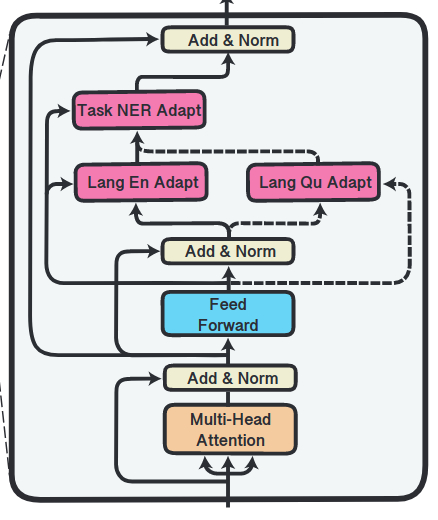
\includegraphics[width=0.86\textwidth]{img/madx.jpg}
%     %    %\vspace{-0.7em}
%     %    \caption{MAD-X. \textcolor{red}{Let's redo this figure?}}
%     %    \label{fig:app_madx}
%     %\end{subfigure}
%      %   \begin{subfigure}[!ht]{0.501\textwidth}
%       %  \centering
%         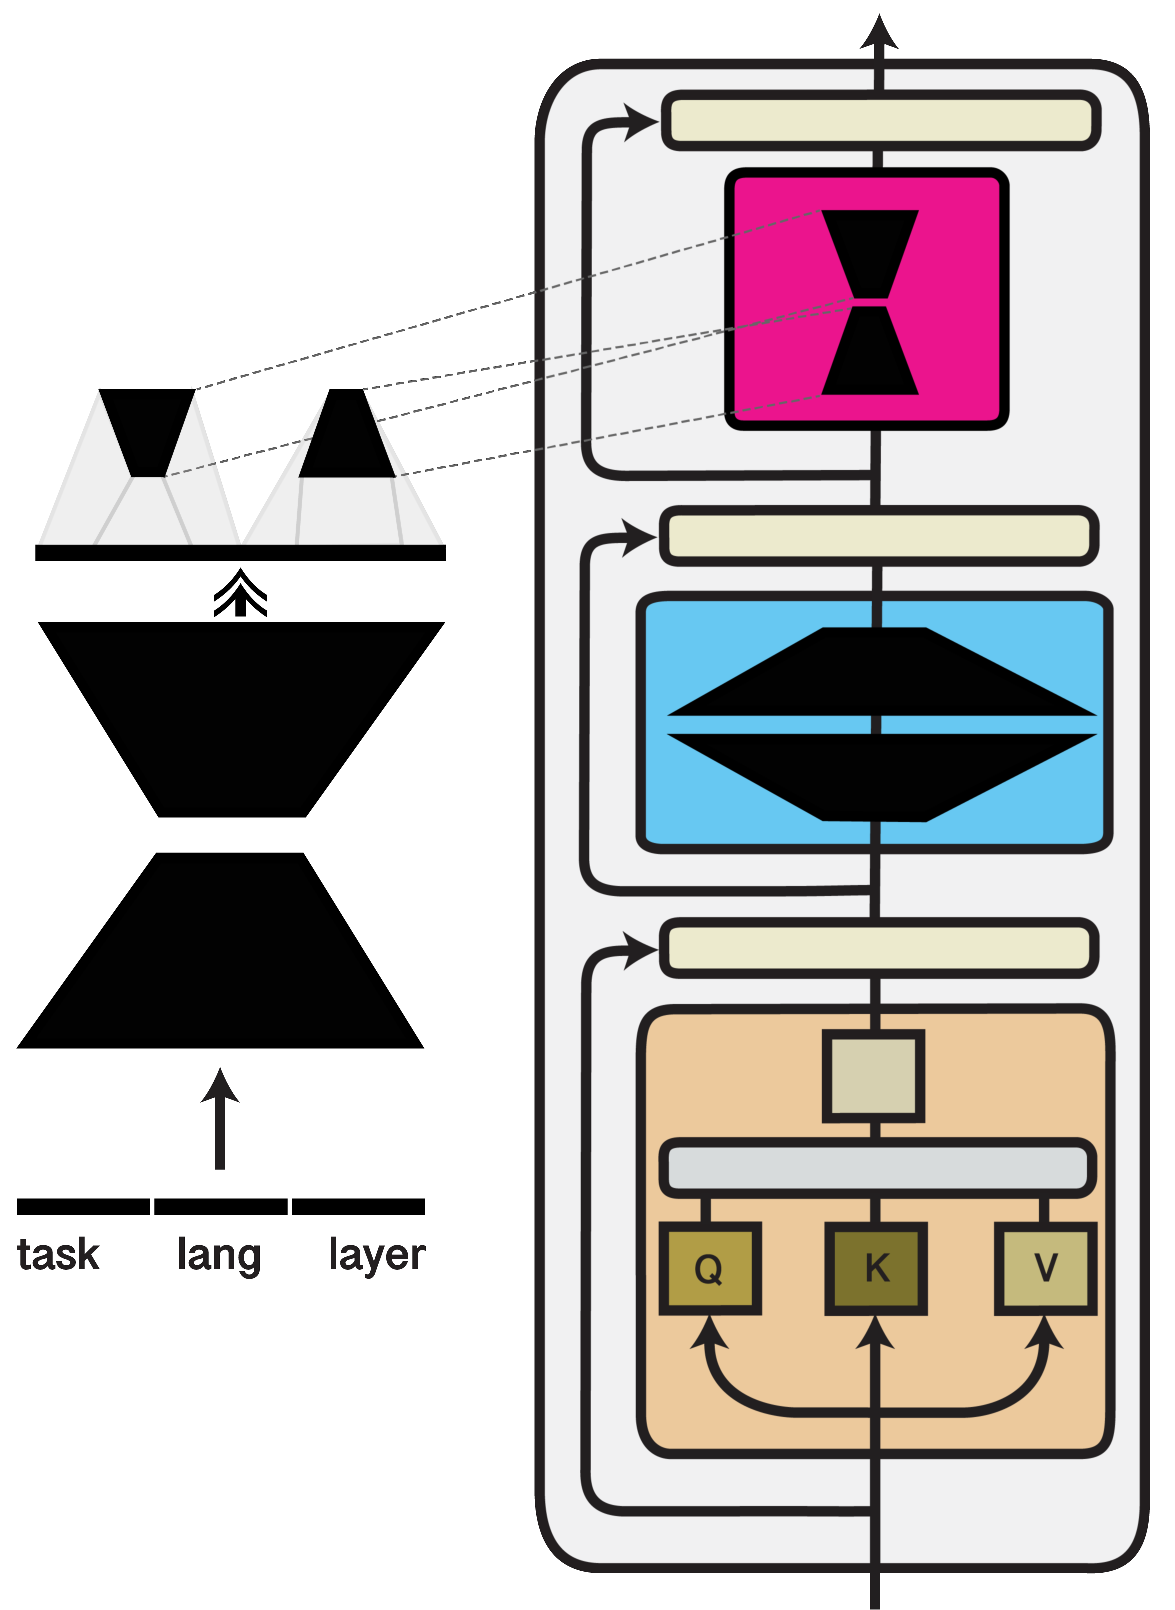
\includegraphics[width=0.3\linewidth, angle=270]{img/hyperx.pdf}
%         %\caption{}
%     %\end{subfigure}
%     \vspace{-0.5mm}
%     \caption{Hyper-X \citep{Ustun:2022hyperx}: an example application of contextual module generation where a hyper-network takes the concatenation of task, language and layer embeddings as input and generates a flat parameter vector that is further reshaped into an adapter module within each Transformer layer. Learning independent layer embeddings \citep{Ansell2021MADG} (i) enables information sharing across layers, and (ii) reduces trainable parameters of the hyper-network by a factor corresponding to the number of layers as a single hyper-network is used across all layers.}
%     \vspace{-0.5mm}
% \label{fig:app_hyperx}
% \end{figure}


\begin{wrapfigure}{r}{0.37\textwidth}
  \begin{center}
    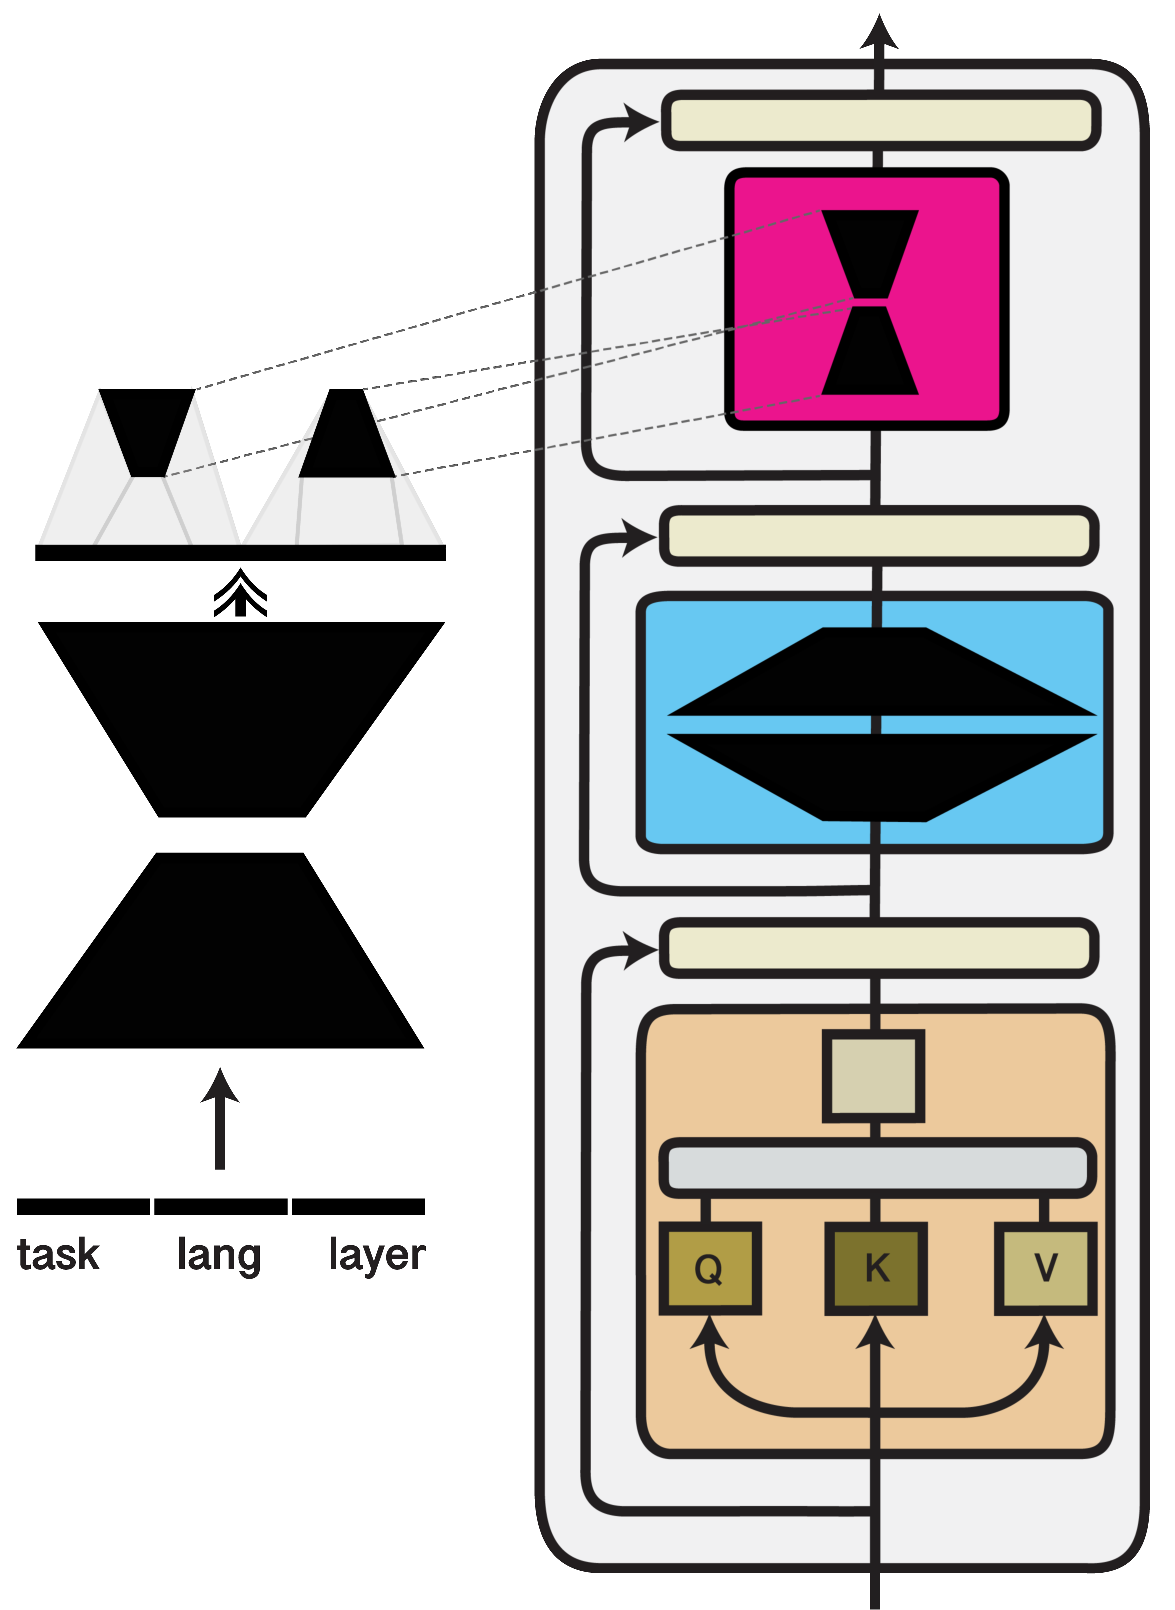
\includegraphics[width=0.3\textwidth]{img/hyperx.pdf}
  \end{center}
  \caption{Hyper-X \citep{Ustun:2022hyperx}: an example application of contextual module generation where a hypernetwork takes the concatenation of task, language and layer embeddings as input and generates a flat parameter vector. This is further reshaped into an adapter module within each Transformer layer. Learning independent layer embeddings and sharing a single hypernetwork across all layers \citep{Ansell2021MADG} (i) enables information sharing across layers, and (ii) reduces trainable parameters of the hyper-network by a factor corresponding to the number of layers.}
  \label{fig:app_hyperx}
\end{wrapfigure}

NMT focuses on translation as a single task and modularity was exploited mainly to carve language-specific and/or domain-specific modules that can support multilingual and multi-domain systems, respectively. In more general cross-lingual transfer setups, the aim is to transfer large models \citep{Devlin:2019bert,conneau-etal-2020-unsupervised} fine-tuned \textit{for any task} (e.g., sequence labelling tasks such as NER, text classification tasks such as NLI, sentiment analysis or intent detection for dialogue systems) on one or more source languages (where such task annotations exist) to one or more target languages \citep{Hu:2020xtreme,Ruder:2021xtremer}. Ideally, the transfer should be achieved without fine-tuning the full large model \citep{Hu:2020xtreme}, which either results in catastrophic forgetting and negative interference, or requires the creation of separate model copies for each task.


The idea of training \textit{language modules} thus largely follows what already outlined for MT in \S\ref{ss:nmt}, with the addition of another set of dedicated modules that aim to capture task-related knowledge: \textit{task modules}. Such language modules and task modules can then be combined to \textbf{1)} favour zero-shot cross-lingual transfer for particular source-target directions \citep{pfeiffer-etal-2020-mad,Ansell2021MADG,ansell2021composable,Parovic2022BADX}; \textbf{2)} provide extra capacity to low-resource languages under-represented (or even not covered) in the large multilingual models such as mBERT or XLM-R \citep{Pfeiffer2021UNKs,Pfeiffer2022Lifting,ponti-etal-2020-xcopa,Faisal:2022arxiv}, independently from task knowledge; and \textbf{3)} enable handling unseen language--task or even language--domain--task configurations \citep{ponti-etal-2021-parameter,Stickland2021MultilingualDomainAdapt}. 


%For instance, disentangling information into dedicated language modules allows us to combine task modules trained with annotated data available only in source languages with target language modules. Exactly this principle is at the heart of modular cross-lingual transfer as demonstrated in  with the MAD-X framework \citep{pfeiffer-etal-2020-mad}. 

As an example of zero-shot cross-lingual transfer, the original MAD-X framework \citep[Figure~\ref{fig:CaseStudy:MADX}]{pfeiffer-etal-2020-mad} relies on bottleneck adapters to implement language and task modules: In particular: \textbf{1)} Language modules are inserted into each layer of the original neural model and are fine-tuned on (unsupervised) data of the particular language (e.g., via Masked Language Modelling) while the weights of the original model are kept fixed. \textbf{2)} After obtaining language modules, task modules are \textit{stacked} on top of the source language module(s) and are fine-tuned relying on the task objective and task-annotated data in the source language(s), while both the original model \textit{and} language modules are kept fixed. \textbf{3)} At inference, source language module(s) are replaced with the desired target language module while retaining the task module: this enables zero-shot task inference in the target language.

Recent work has introduced a spectrum of variations and enhancements to this core idea. For instance, inspired by the bilingual `translation direction' adapters for NMT systems (\S\ref{ss:nmt}), \cite{Parovic2022BADX} learn bilingual adapters instead of single language adapters to boost transfer for a particular language pair. \cite{Faisal:2022arxiv} and \cite{Chronopolou:2022arxiv} learn language family adapters to reduce data sparsity for low-resource languages and capitalise on language similarity and cross-language sharing. \cite{Stickland2021MultilingualDomainAdapt} decouple language and domain knowledge into dedicated modules (see also \S\ref{sec:domain_adap} later). %\cite{Vidoni:2020arxiv} aim to maximise the injection of new knowledge into the modules through the introduction of an auxiliary loss based on orthogonality constraints \citep{Romera:2012orthogonality}. 
Further, \cite{ansell2021composable} implement dedicated modules as sparse sub-networks, the so-called language and task masks, which can be composed with the base model via parameter composition. Following the analogy between language-specific and bilingual adapters, instead of learning separate language and task sub-networks, \cite{Foroutan2022Discovering} learn dedicated task--language sub-networks, demonstrating the variance in the extracted sub-networks across different task--language combinations. The use of such language sub-networks as language modules, even without dedicated task modules, improves cross-lingual transfer for dependency parsing when used within a meta-learning setup \citep{Choenni:2022arxiv}. \citet{litschko-etal-2022-parameter} compare sparse sub-networks and bottleneck adapters for transferring ranking functions for information retrieval tasks across languages and find them both superior to full model fine-tuning.

Finally, a body of work again focuses on `contextually generating' the modules via hypernetworks, aiming to increase efficiency and benefit from connections between different languages \textit{and} tasks. A representative example is the Hyper-X framework \citep{Ustun:2022hyperx} provided in Figure~\ref{fig:app_hyperx}, where the module parameter generation is conditioned on the (disentangled) task and language, and additionally on the index of the Transformer layer where the generated module is inserted. Each task and language are parameterised via separate embeddings, which enables adaptation to any task--language combination, where these embeddings are low-dimensional vectors which are learned together with the parameters of the hypernetwork (see Figure~\ref{fig:app_hyperx} again). The framework thus leverages supervision and positive transfer from both multiple tasks and languages. Hyper-X can be seen as a more general variant of a series of precursors backed by the idea of contextual generation: \citet{ponti-etal-2021-parameter} condition the hypernetwork on both task and language embeddings but generates only the model's classifier head. Other methods generate modules but condition the hypernetwork only on tasks in a monolingual setup \citep{mahabadi2021parameter} or only on languages in a cross-lingual transfer setup \citep{Ustun2020,Ansell2021MADG}.

%Analyzing language subnetworks (building on LT-SFT): \cite{Foroutan2022Discovering}
%Mention language family adapters \cite{Chronopolou:2022arxiv}.
%Information retrieval \cite{Ma:2022retrieval} \cite{litschko-etal-2022-parameter}

\subsubsection{Domain Adaptation}
\label{sec:domain_adap}
As already hinted at in \S\ref{ss:nmt} and \S\ref{sec:xling-transfer}, dealing with different domains adds another tier to the modular design: domain-specific knowledge might be captured within dedicated \textit{domain modules}.\footnote{For instance, disentangling domain and language information yields benefits for NMT and cross-lingual transfer applications \citep{vilar-2018-learning,cooper-stickland-etal-2021-multilingual,pham-etal-2021-revisiting,Saunders:2022survey}.} This can again be accomplished through similar modular architectures as with language and task adapters. For instance, it is possible to inject domain-specific knowledge into (bottleneck) adapters \citep{Zhang:2021ws,Chronopoulou2022EfficientHierarchical} or to extract sparse domain-specific or task-specific sub-networks \citep{Thompson:2018nmt,ke-etal-2021-adapting} for multi-domain and multi-task learning. Mixture-of-experts also enable multi-domain joint learning as well as domain adaptation \citep{Guo:2018emnlp,Zhang:2022metadmoe}. Similar strategies have also been used in multi-domain and cross-domain speech processing and computer vision applications (see \S\ref{ss:speech} and \S\ref{ss:cv} later).

In domain adaptation, it is common to combine both shared parameters and domain modules that are learned jointly \citep{Bousmalis2016}. Beyond this standard setting, many approaches employ additional regularisation terms. The most common are \textbf{1)} a domain-adversarial loss on the shared parameters in order to encourage them to be domain-invariant \citep{ganin2016domain,chen-cardie-2018-multinomial}; \textbf{2)} an orthogonality constraint on the domain modules to ensure that they capture different information \citep{baktashmotlagh2013unsupervised,kim-etal-2017-adversarial}; and \textbf{3)} similarity constraints that bring representations of similar modules close together \citep{Bousmalis2016}.

%Domain and language information \cite{cooper-stickland-etal-2021-multilingual} \cite{vilar-2018-learning} \cite{Saunders:2022survey} \cite{pham-etal-2021-revisiting}

%\seb{Two more things that come to mind that we are not currently discussing: A general comparison between different methods and a recommendation which one is currently best to use. Could we run a comparison here using the AdapterHub? And a section about things that are important but do not clearly fall into any of the previous categories. For instance, common loss functions to encourage modularity (things like orthogonality constraints).}

%\subsection{Other Applications in NLP}
\subsubsection{Knowledge Injection}
\label{ss:knowledge_injection}
Naturally, dedicated modules can also be assigned to inject and store external knowledge (e.g., from manually curated external knowledge bases), which can then interact with language, domain, or task knowledge. This idea has been explored with diverse external knowledge sources. For instance, \citet{lauscher-etal-2020-common} aimed at complementing the distributional knowledge of large language models with conceptual and commonsense knowledge from ConceptNet \citep{Speer:2017conceptnet}. The external knowledge was captured within dedicated bottleneck adapters: they were fine-tuned via language modelling on synthetically created sentences from random walks over the ConceptNet graph structures. \cite{majewska-etal-2021-verb} stored verb-related knowledge from VerbNet \citep{schuler2005verbnet}, a human-created verb classification repository, into bottleneck adapters, and demonstrated its usefulness in a range of tasks that require understanding of verb semantics. Along similar lines, \citet{wang-etal-2021-k} offered a generalisation of these approaches where different knowledge sources (e.g., Wikipedia, WikiData) are mapped to different dedicated adapters, which can be aggregated according to the task at hand. The same idea has been explored by \citet{Lu:2021knowledge} in the biomedical domain, where the main knowledge sources were the UMLS Metathesaurus graph \citep{bodenreider2004unified} and biomedical Wikipedia articles. \citet{Lu:2021knowledge} also introduce another component, the so-called knowledge controller, which can be seen as a standard attention-based function aggregator from \S\ref{sec:compositionality:function}. 

\begin{wrapfigure}{r}{0.27\textwidth}
  \begin{center}
    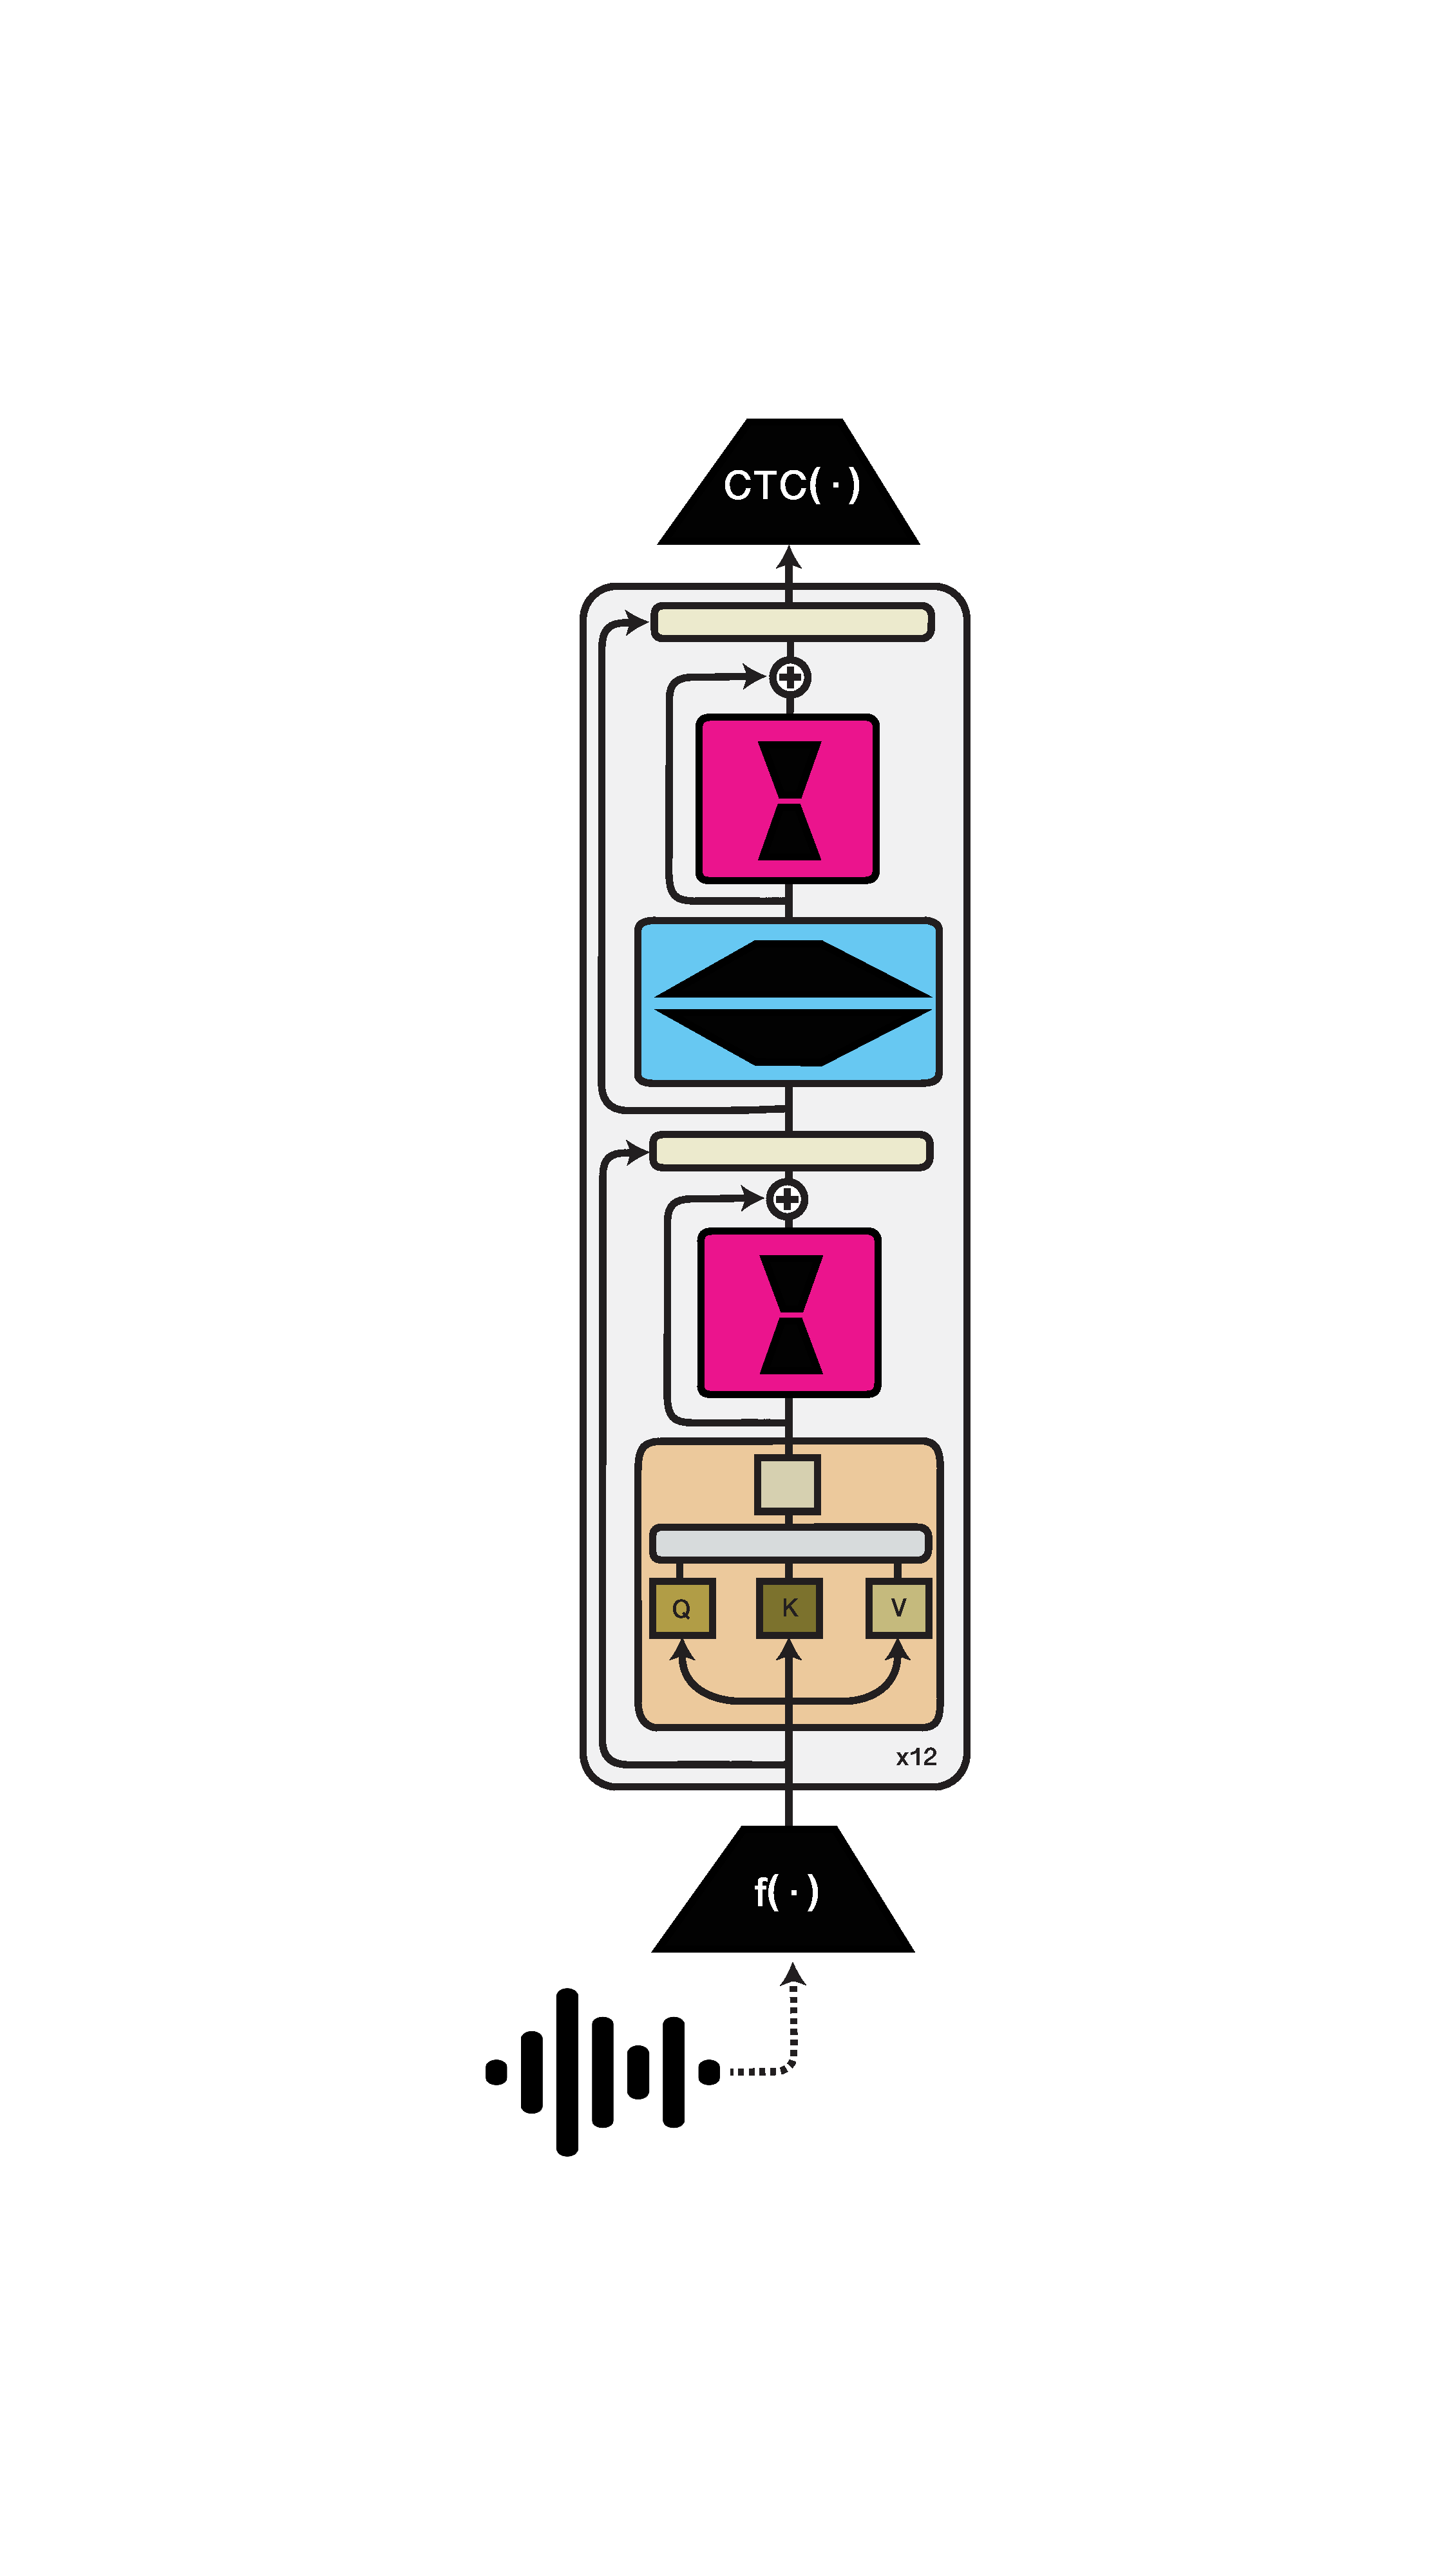
\includegraphics[width=0.17\textwidth]{img/wav2vec.pdf}
  \end{center}
  \caption{The structure of the wav2vec 2.0 model with task-specific bottleneck adapters for parameter-efficient ASR fine-tuning from \citet{Thomas:2022speech};
  %a similar architecture is used by other parameter-efficient ASR methods \citep[\textit{among others}]{Sathyendra:2022speech,Chen:2022speech}. 
  $f(\cdot)$ denotes a convolutional encoder followed by 12 standard Transformer encoder blocks. For downstream ASR a linear classifier, $CTC(\cdot)$, is applied to the final encoder output.}
   \label{fig:app_speech}
\end{wrapfigure}

Finally, \citet{lauscher-etal-2021-sustainable-modular} learned bottleneck adapters without manually curated external data, with the focus on model debiasing: the debiasing adapters were fine-tuned via standard language modelling on a counterfactually augmented corpus. 

%\cite{wang-etal-2021-k} \cite{majewska-etal-2021-verb} Biomedical: \cite{Lu:2021knowledge} (they also have a `routing adapter')


%%Knowledge extraction: \cite{Newman:2022iclr} (also tried MoE)

%\paragraph{Task-Oriented Dialogue Systems}

\subsubsection{Speech Processing}
\label{ss:speech}
The use of modular deep learning for speech processing applications closely matches the ideas already exposed for NLP tasks. The landscape of the possible modular designs is exactly the same, where the only crucial differences are (i) the choice of the underlying large model, and (ii) the corresponding objective functions used to inject the specialised knowledge into the modules. For instance, the typical choice of the base model for automatic speech recognition (ASR) applications is one from the wav2vec family \citep{Baevski:2020wav2vec,Babu:2022xlsr}, while the ASR-oriented objective function is the standard Connectionist Temporal Classification (CTC) loss \citep{Graves:2006ctc}. The high-level modular structure remains the same, as illustrated in Figure~\ref{fig:app_speech} with an example from \citet{Thomas:2022speech}, which utilises standard bottleneck adapters.

% \begin{figure}[!t]
%         \centering
%         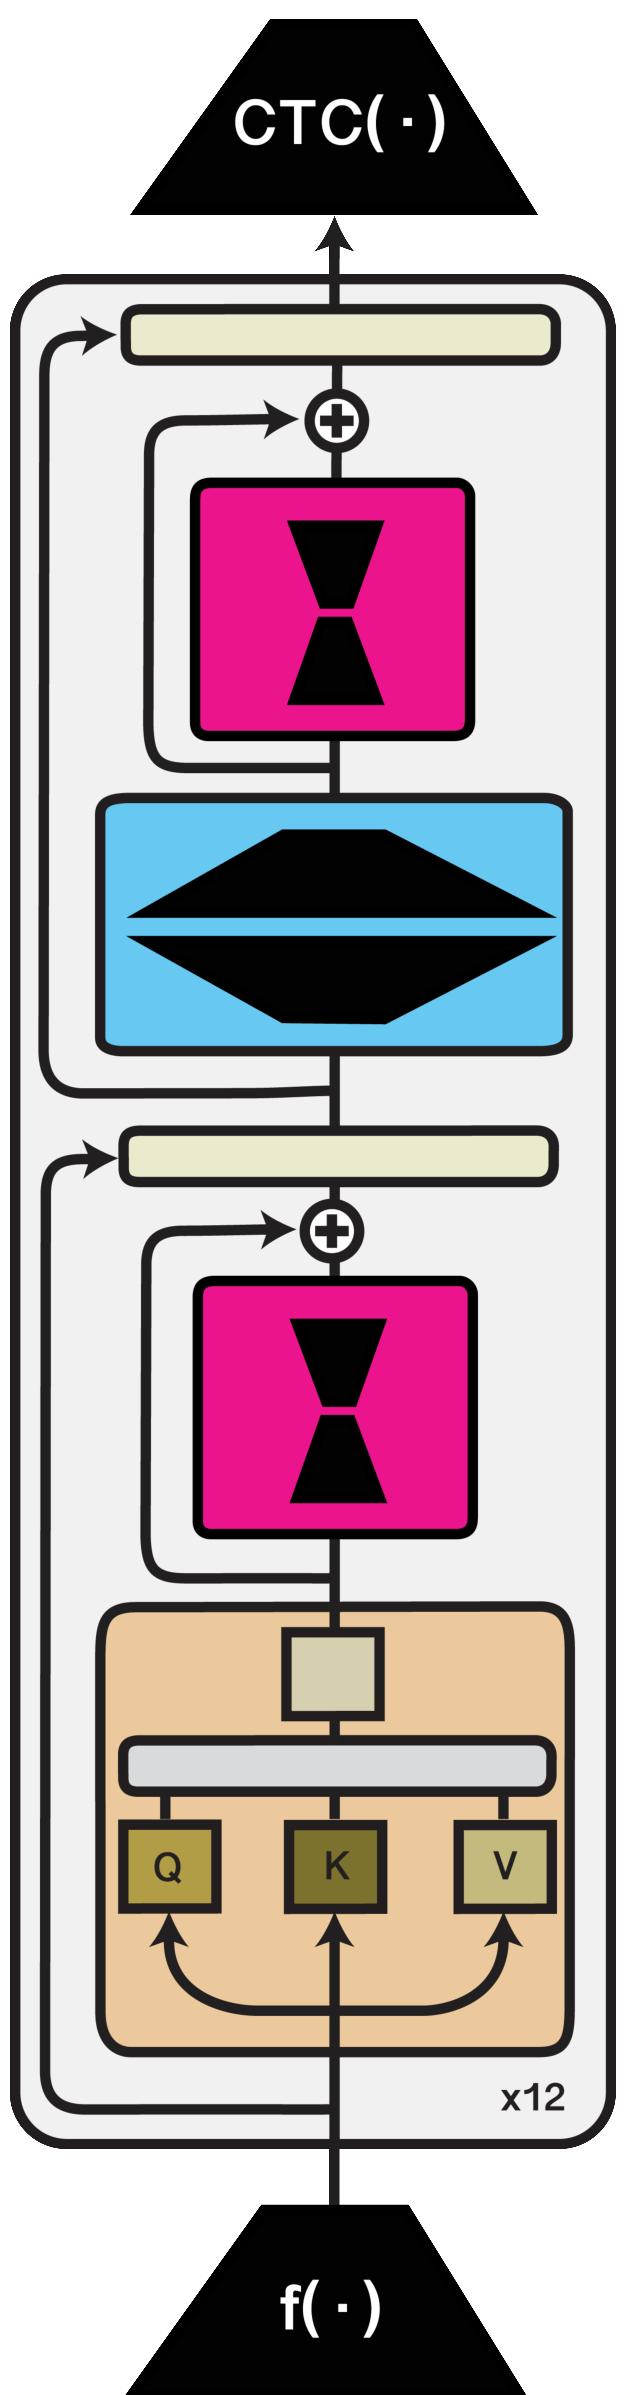
\includegraphics[width=0.15\textwidth,angle=270]{img/speech.pdf}
%         %\vspace{-0.7em}
%         \caption{The structure of the wav2vec 2.0 model with task-specific bottleneck adapters for parameter-efficient ASR fine-tuning from \citet{Thomas:2022speech}; a similar architecture is used by a plethora of other parameter-efficient ASR methods \citep[\textit{among others}]{Sathyendra:2022speech,Chen:2022speech}. $f(\cdot)$ denotes a convolutional encoder followed by the standard 12 Transformer encoder blocks. For downstream ASR a linear classifier, $CTC(\cdot)$, is applied to the final encoder output.}
%         \label{fig:app_speech}
% \end{figure}


While in theory a large variety of possible modular configurations from \Cref{sec:nature_modularity}-\Cref{sec:training} can be applied to diverse speech processing tasks, the majority of current work in the area has indeed focused on the use of bottleneck (sequentially placed) adapters for ASR in monolingual and multilingual contexts. Before that, the concept of modularity can be traced to the work of \citet{Swietojanski:2016taslp}, where the model re-weights hidden units using small amounts of unsupervised data to better adapt to a particular speaker of an environment. More recently, bottleneck adapters have been used to perform ASR adaptation to atypical and accented speech \citep{tomanek-etal-2021-residual}, unseen speakers with limited adaptation data \citep{Wang:2022speech,Eeckt:2022speech,Chen:2022speech}, new domains and manners of speaking (e.g., children's speech) \citep{Fan:2022speech,Zhu:2022speech}, or to perform further model customisation to specific speakers \citep{Biadsy:2022speech,Sathyendra:2022speech} and for multilingual learning \citep{Kannan:2019interspeech,Hou:2022speech}. A notable exception, not resorting to adapter layers, is the method of \citep{Winata:2020speech} which aims to learn low-rank modules (\S~\ref{sec:nature_modularity:parameter_composition}), akin to the idea of LoRA \citep{hu2021lora}, for end-to-end ASR.



Multi-task (where `task' can e.g. refer to different languages, domains, speakers, or accents) ASR setups have also witnessed the usage of mixture-of-experts, closely following the basic ideas already discussed for NMT (\S\ref{ss:nmt}) where different languages are assigned their dedicated modules through fixed routing. For instance, in speech processing, MoEs have been applied to multilingual ASR and cross-lingual ASR transfer \citep{Bai:2022speech,Gaur:2021speechmoe,Kumatani:2021arxiv}, while \cite{you2022speechmoe2} propose MoE for ASR with learned routing.

Beyond ASR, bottleneck adapters have also been used for speech translation \citep{le-etal-2021-lightweight}. Most recently, modular adapter-based approaches have been applied to text-to-speech methods (TTS) \citep{Hsieh:2022tts,Morioka:2022tts}, aiming to extend standard large multi-speaker TTS models such as FastPitch \citep{Lancucki:2021fastpitch} to new speakers without compromising the TTS quality for the seen speakers. From a high-level perspective, one can see a direct analogy of this goal to the objectives in the MT literature of extending multilingual MT systems to unseen languages without compromising seen languages (see \S\ref{ss:nmt} again).




\subsubsection{Computer Vision and Cross-Modal Learning}
\label{ss:cv}
In computer vision, similar to NLP and speech processing (\S\ref{ss:speech}), dedicated modules are again used to enable parameter-efficient fine-tuning across multiple tasks and domains \citep[\textit{among others}]{Rusu2016Progressive,Rebuffi2018Adapters2,Berriel:2019iccv,He:2022arxiv}. The core difference, again, is the choice of the actual neural architecture for the underlying model as well as for the modules: e.g., residual adapters \citep{Rebuffi2017Adapters1} consisted of simple $1 \times 1$ convolutions combined with the base ResNet neural model \citep{He2016ResNet} while other work learned task-specific convolutional filters \citep{newell2019feature,bragman2019stochastic}.
More recent work aims to exploit modular architectures from NLP (e.g., sequential or parallel adapters, LoRA, prefix tuning) with pretrained Vision Transformer (ViT) architectures \citep{dosovitskiy2020image}: e.g., \citet{He:2022arxiv} run a comparative empirical analysis of various modular architectures for vision tasks, while \citet{Chen:2021neurips} rely on sparse sub-networks. %as modules.

Modular design lends itself naturally to cross-modal and multi-modal applications, where different modalities may be captured by modality-specific parameters and routing can also be modality-conditioned. For instance, in multilingual vision-and-language (V\&L) settings, it is possible to conduct inference in languages that lack labelled task examples. In fact, language knowledge is again disentangled from the task and modality knowledge, and the knowledge for different input modality streams can be captured in dedicated modules. This idea has been heavily explored in recent work in multi-modal multi-task scenarios, both in monolingual \citep{Sung:2022modal} and multilingual contexts \citep{bugliarello2022iglue,pfeiffer-etal-2022-xgqa}, for tasks such as image captioning \citep{Zhou:2022modal,Gao:2021modal}, text-to-image generation \citep{Maharana:2022modal}, visual question answering \citep{Liu:2022delving,Sung:2022modal}, visual reasoning \citep{liu-etal-2021-visually}, etc. For instance, Flamingo \citep{alayrac2022flamingo} uses frozen pretrained vision and language models, and only trains adapter layers to handle sequences of arbitrarily interleaved visual and textual data. It is trained with a sequence modelling objective on Web-scale data \citep{li2021align} and displays impressive zero-shot and few-shot capabilities. \cite{pfeiffer-etal-2022-xgqa} use adapter modules to equip multilingual text-only models with the ability to also process the visual modality, as well as to equip monolingual multi-modal models to deal with input from multiple languages. \citet{Papalampidi:2022modal} rely on hierarchical adapters (akin to hierarchical representation aggregation discussed in \Cref{sec:compositionality}) for the task of summarising long videos into textual descriptions. \citet{Pan:2022modal} demonstrate that modular design also helps in image-to-video transfer tasks: they use adapter modules to equip a large image-based model without temporal knowledge with the ability to reason about dynamic video content. 

We note that in this survey, we aim to list some exemplary applications and draw parallels between different yet similar application areas such as NLP, speech processing, and computer vision. While we acknowledge that there exists a wealth of other work in these areas, we have no pretence of exhaustiveness.

%\cite{Berriel:2019} \cite{Chen:2022visiontransformer} \cite{riquelme2021scaling} \cite{Rebuffi2018Adapters2} \cite{He:2022parameer}


%Image-to-video: \cite{Pan:2022modal}
%V\&L: \cite{Sung:2022modal} \cite{pfeiffer-etal-2022-xgqa} \cite{Zhou:2022modal} \cite{Gao:2021modal} \cite{Papalampidi:2022modal} (long video-to-text summarisation; hierarchical adapters)
%TTI: \cite{Maharana:2022modal}

%% (Removed, this is an old comment)
%%\seb{Reinforcement Learning.\citet{heess2016learning} and \citet{devin2017learning} learn modular policies for robotic learning. See section 2.3.2 of \citep{crawshaw2020multi}}

% In Progressive Networks \citep{Rusu2016Progressive}, each module is a separate neural network consisting of multiple layers. Each layer in a new module is additionally connected to the preceding layer of all previously learned modules. Subsequent work \citep{Schwarz2018progress} distills the information of the new module into the existing module at the cost of modularity. 

%\ivan{This is not related to RL}
\subsubsection{General Considerations}
\label{sec:app_summary}
While a full-fledged comprehensive empirical study of the plethora of modular architectures across various application tasks and areas is still lacking, there exist initiatives such as the publicly available AdapterHub platform \citep{pfeiffer-etal-2020-adapterhub}: it provides (re)implementations of representative modular NLP architectures, within a unified framework tied to HuggingFace Transformers \citep{wolf2019huggingface}. Among others, AdapterHub includes representatives of each computation method in \Cref{sec:nature_modularity}: LoRA \citep{hu2021lora} (i.e., low-rank parameter composition), prefix tuning of \cite{Li2020PrefixTuning} (input composition) and a number of bottleneck adapter configurations (function composition). %The implemented architectures are typically verified on the standard GLUE tasks, which offers partial insight into their relative performance and capability across standard NLP tasks. 
The existence of AdapterHub delineates another crucial advantage of modularity: \textit{reusability} of existing, already fine-tuned modules which can be (re)combined with the large neural models. In short, any practitioner can share or reuse a module specialised for a particular purpose (e.g., capturing specific task or language knowledge) with the community, facilitating community-wide sharing and thus avoiding time- and energy-costly repetitions of the same fine-tuning procedure.\footnote{The (concept of) reusability enabled by the modular design also positively impacts energy consumption \citep{strubell-etal-2019-energy}, making an important leap towards Green(er) AI \citep{Schwartz:2020greenai}.} As discussed in \Cref{sec:routing}, one can observe initiatives such as AdapterHub as continuously updating community-distributed multi-task models.

The discussion in this section also points to a more general principle: different end-goals even within the same end-application (e.g., NMT, cross-lingual transfer, domain adaptation) require rethinking the actual modular design, and the desired level and nature of modularity. For instance, if the goal in NMT (or cross-lingual transfer) is to boost performance for a particular translation or transfer direction, it might be useful to trade off some modularity for a better final performance by replacing language-specific monolingual modules with bilingual modules \citep{Bapna2019Adapters,Parovic2022BADX}. On the other hand, if the goal is to enable zero-shot or few-shot translation or transfer, the design with monolingual modules might be a better choice. In another example, if the focus is on MT or transfer for a particular low-resource language, the model designer should enable positive transfer to that language by `opening' the flow of information from a module storing knowledge on high-resource languages similar to the target language if such languages exist (e.g., from Spanish to Galician) \citep{ustun-etal-2021-multilingual}, or by learning modules for families or groups of similar languages \citep{Chronopolou:2022arxiv,Faisal:2022arxiv}. Analogously, related domains can also be grouped and hierarchically organised to enable positive transfer for domain adaptation \citep{Chronopoulou2022EfficientHierarchical}.

Other practical desiderata may also influence the selection of the actual modular design. If the final task performance is paramount, larger modules might be preferred, e.g., in order to offer enough extra capacity to store the wealth of language-specific information \citep{ansell2021composable}. However, if model compactness is paramount, the criterion for choosing a specific design is instead the trade-off between efficiency (in terms of parameters and/or train and test time) and task performance; the optimisation of this trade-off has been the focus of recent research \citep{Rueckle2021AdapterDrop,Mahabadi2021Compacter,mahabadi2021parameter,Sun:2022bbtv2}. In another example, if time efficiency during inference is a crucial requirement (e.g., real-time ASR in dialogue systems, low latency for information search systems) parameter composition methods such as sparse subnetworks or low-rank composition methods may be preferred over function composition methods as the latter increase the number of computations required during the forward pass, (see Table~\ref{tab:computation_function_comparison}). In yet another example, if storage requirements are a critical constraint, one cannot resort to huge mixture-of-expert models where billions of parameters must be stored \citep{Lepikhin2021GShard}.

\subsection{Task Generalisation}
\label{ssec:task_gen}
The diverse applications of modular deep learning covered so far almost exclusively focus on learning modules associated with (arguably) well-formed and interpretable `units of knowledge' such as languages, tasks, domains, dialects, accents, and speakers. However, modularity might also be achieved when such units are \textit{unknown}. This relies on jointly learning arbitrarily sized inventories of so-called latent \textit{skills} and a learned routing function (\S~\ref{sec:routing:learned}). Since such skills are learned end-to-end on a mixture of data from multiple tasks, they are often not straightforwardly interpretable. On the other hand, since arbitrary subsets of skills can be combined and each skill can be updated locally, these modular neural architectures are ideal for systematic generalisation to new tasks \citep{Zhang2022SkillNet,ponti2022combining}. 

In fact, another fundamental application in transfer learning is achieving zero-shot or few-shot generalisation to new tasks, where test examples are not i.i.d.\ with respect to training examples. The general experimental setup involves disjoint sets of training and test tasks. A model is pre-trained through multi-task learning on training tasks and then adapted to each new test task based on zero or few data points. Common examples of evaluation benchmarks for this setting include CrossFit \citep{ye-etal-2021-crossfit}, the T0 task suite \citep{sanh2022multitask}, or Natural Instructions \citep{mishra-etal-2022-cross}. While a common strategy to tackle this problem is instruction tuning \citep{sanh2022multitask,wei2022finetuned}, where models are fine-tuned prepending the instructions for each task, modular deep learning has emerged as a strong contender \citep{alet2018modular,kudugunta2021beyond,ponti2022combining}.

%\ivan{Note to self - talk about training and inference efficiency; model compactness; hparam optimisations: UniPELT, etc}